% !TEX TS-program = pdflatex

\documentclass[unicode,11pt,notheorems,xcolor=table]{beamer}

\usepackage[T2A]{fontenc}
\usepackage[utf8]{inputenc}
\usepackage[russian]{babel}
\usepackage{amsmath,amsfonts,amssymb,amsthm}
\usepackage{mathtools}
\usepackage{diagbox}

\usepackage{ulem}
\usepackage{tikz, graphicx}
%\usepackage{tkz-graph}
\usetikzlibrary{matrix,arrows,decorations.pathmorphing, arrows.meta,positioning}
\usetikzlibrary{positioning,calc}
\usetikzlibrary{petri}
\usetikzlibrary{decorations.pathreplacing}

%Описание стиля презентации
\usetheme[sidebar=0]{kfmn} 
\setbeamercovered{transparent}

%\definecolor{cyan}{RGB}{240,217,1}
%\definecolor{vgugreen}{RGB}{143,188,103}
%\definecolor{vgured}{RGB}{234,38,40}
%\definecolor{vgublue}{RGB}{53,101,167}



\makeatletter
	\g@addto@macro{\endtabular}{\rowfont{}}% Clear row font
	\makeatother
	\newcommand{\rowfonttype}{}% Current row font
	\newcommand{\rowfont}[1]{% Set current row font
		\gdef\rowfonttype{#1}#1\ignorespaces%
	}
\makeatother

\newcommand{\myunit}{9mm}
\tikzset{
    node style sp/.style={draw,circle,minimum size=\myunit},
    node style ge/.style={circle,minimum size=\myunit},
    arrow style mul/.style={draw,sloped,midway,fill=white},
    arrow style plus/.style={midway,sloped,fill=white},
}

%[0, 6, 8, 8, 10, 5, 6, 10, 8, 10, 10], 

\pgfdeclareimage[height=8mm]{university-logo}{logo-iem.png}
\logo{\pgfuseimage{university-logo}}
%2[0, 11, 10, 8, 11, 5, 11, 11, 8, 11, 10, 11],

\titlepicture{
	\begin{tikzpicture}[y=1.4cm,overlay,rotate=8]
	\coordinate (O) at (-3cm,0.9cm);
	\filldraw[thick,draw= vgublue, fill=vgublue!20!white] (0,0) circle[radius=4.2cm];
	\clip (0,0) circle[radius=4.2cm];
	\draw (-1.5,1.5) node{
	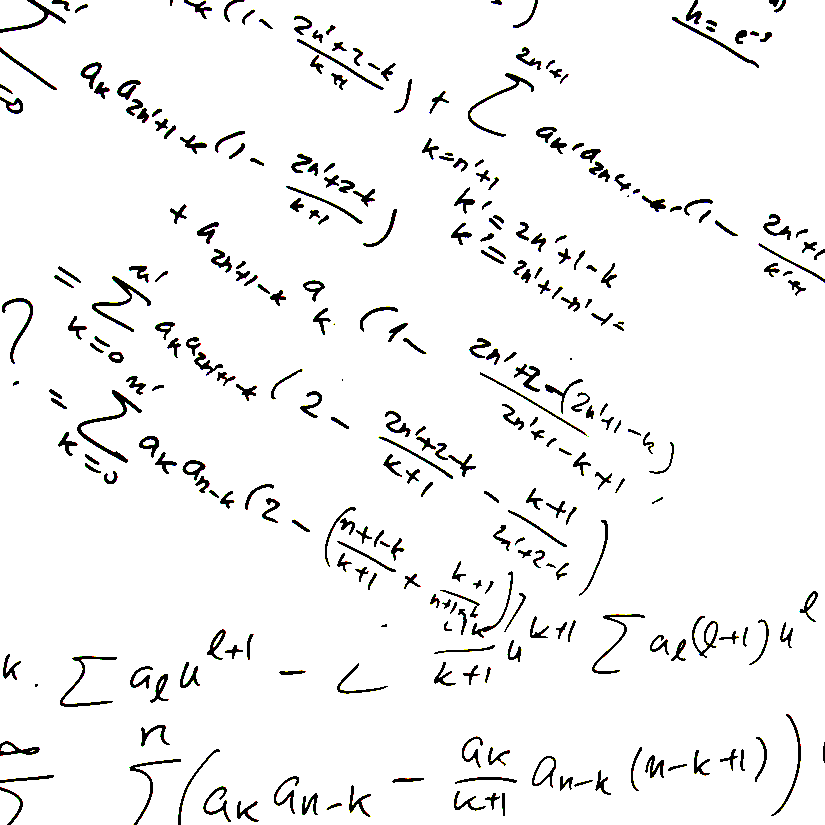
\includegraphics[width=8cm]{titlepic.png}
	};
\end{tikzpicture}
}

\usepackage[math]{iwona}

\newcommand{\hplus}{\mathbin{\hat+}}
\newcommand{\hdot}{\mathbin{\hat\cdot}}
% Описание теорем
\newtheorem{theorem}{Теорема}
\newtheorem{seq}{Следствие}
%%

%\VKR
\LECT % можно ещё лекцию забацать.
%\REPORT % можно ещё лекцию забацать.

%\titlepicture{
%%	\begin{tikzpicture}[overlay]
%%			\draw[opacity=0.4]  (-0.3,1.8) node {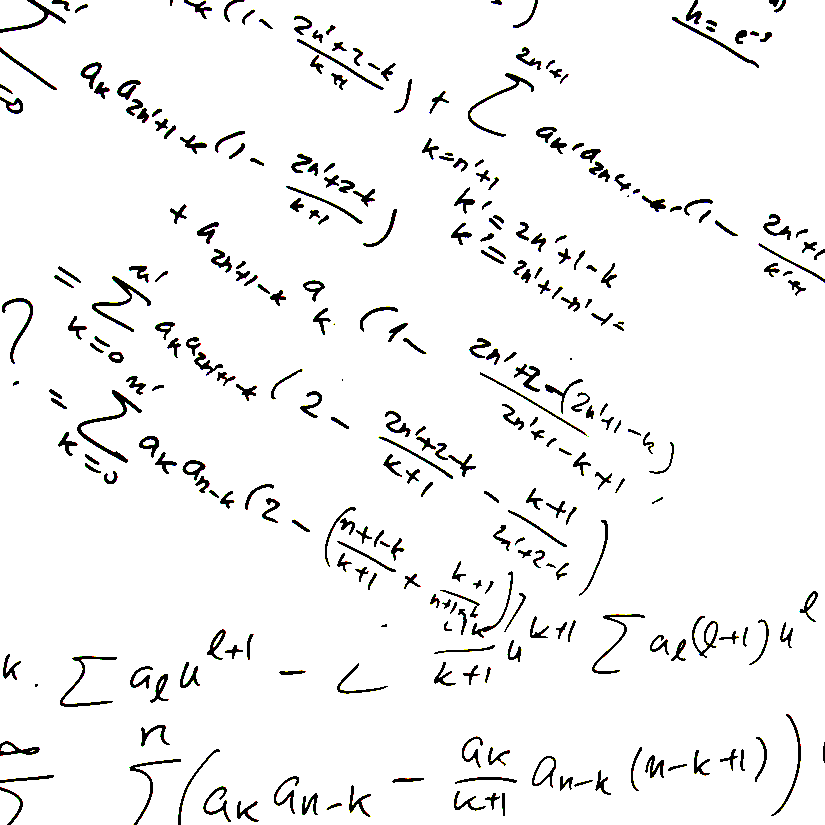
\includegraphics[width=3.5cm]{titlepic.png}};
%%	\end{tikzpicture}
%}

% Титульный лист теорем
\author[Д.\,В. Чупраков]{канд.\,физ.-матем.\,наук, доцент Д.\,В. Чупраков\\[6pt] usr10381@vyatsu.ru}

\institute[ВятГУ]{ФГБОУ ВО Вятский государственный университет}

\department{Факультет экономики и финансов}

\title[Лекция~6. Линейные задачи. Часть~4 из 4]{
	Введение в экономико-математическое моделирование\\[12pt]
	Лекция 6. Линейные задачи--4}
\subtitle{Теория двойственности и транспортная задача}

\date{15 октября 2020 г.}


%\setbeamercolor{coloredboxstuff}{fg=yellow,bg=white!10!blue}

\setbeamercovered{invisible}


\tikzset{
	 myarrow/.style={->, >=latex', shorten >=1pt, thick}
}



\tikzset{add/.style n args={4}{
    minimum width=6mm,
    path picture={
        \draw[black] 
            (path picture bounding box.south east) -- (path picture bounding box.north west)
            (path picture bounding box.south west) -- (path picture bounding box.north east);
        \node at ($(path picture bounding box.south)+(0,0.13)$)     {\tiny #1};
        \node at ($(path picture bounding box.west)+(0.13,0)$)      {\tiny #2};
        \node at ($(path picture bounding box.north)+(0,-0.13)$)        {\tiny #3};
        \node at ($(path picture bounding box.east)+(-0.13,0)$)     {\tiny #4};
        }
    }
}

\tikzset{bigadd/.style n args={4}{
    minimum width=20mm,
    path picture={
        \draw[black] 
            (path picture bounding box.south east) -- (path picture bounding box.north west)
            (path picture bounding box.south west) -- (path picture bounding box.north east);
        \node at ($(path picture bounding box.south)+(0,0.5)$)     { #1};
        \node at ($(path picture bounding box.west)+(0.5,0)$)      {#2};
        \node at ($(path picture bounding box.north)+(0,-0.5)$)        {#3};
        \node at ($(path picture bounding box.east)+(-0.5,0)$)     {#4};
        }
    }
}
\begin{document}


\maketitle

\begin{frame}{Структура лекции}
	\tableofcontents
\end{frame}


\section{Двойственная ЗЛП}
\begin{frame}{}{}
	\centering 
	\Large Двойственная задача линейного программирования
\end{frame}

\begin{frame}{Ситуация}
	
	Предприятие производит продукцию $n$ видов из сырья $m$ видов. 
	Какое количество продукции $x_1, x_2,\ldots, x_n$ необходимо произвести, чтобы при заданных стоимостях $c_1, c_2,\ldots c_n$ единицы продукции и объемах имеющегося сырья $b_1, b_2, \ldots b_m$ максимизировать доход от продажи продукции.

\pause
\bigskip
\begin{block}{Некоторое предприятие решило перекупить это сырье.}


\begin{itemize}
\item 
	Продавцу сырья сделка выгодна, если доход от продажи сырья превзойдет доход от реализации продукции.
\item 
	Покупателю хочется купить сырье по минимальной цене.
\end{itemize}

\alert{Какие цены на сырье удовлетворят обе строны?}
\end{block}


%\pause
%
%\begin{block}{Двойственная задача:}
%	Какова должна быть цена единицы каждого из~$m$ ресурсов, чтобы при заданных количествах ресурсов $b_1, b_2, \ldots b_m$ и~величинах стоимости единицы продукции $c_1, c_2,\ldots c_n$ минимизировать общую стоимость затрат? 
%\end{block}


%Поясним некоторые вопросы. 
%На этапе постановки задачи производится анализ с целью ответить на вопросы:
%\begin{itemize}
%\item Что будет, если \ldots?
%\item Что надо, \ldots чтобы \ldots ?
%\end{itemize}
%Анализ с целью ответа на первый вопрос называется вариантным анализом, на второй~--- решениями по заказу. 
%
%Вариантный анализ бывает следующих видов: 
%Параметрическим будем называть такой анализ, который заключается в решении задачи при различных значениях некоторого параметра; 
%Под структурным анализом будем понимать решение задачи оптимизации при различной структуре ограничений; 
%Многокритериальный анализ – это решение задачи по разным целевым функциям; Если исходные данные, используемые при решении задачи, зависят от соблюдения дополнительных условий, то такой анализ называется анализом при условных исходных данных.
%
%Во вторую группу – решения по заказу – входят задачи, целью которых является решение задачи оптимизации при заданных значениях: переменных, левых частей ограничений, целевой функции. Кроме анализа, выполняемого на этапе постановки задачи, мощным средством, помогающим принять решение, является анализ полученного оптимального плана. 
\end{frame}

\begin{frame}{Формализация. Прямая задача}{}
\small
$$
\begin{array}{|>{\columncolor{cyan!40}}l|c|c|c|c|>{\columncolor{green!40}}c||>{\columncolor{yellow!40}}c|}
	\rowcolor{cyan!40}\hline
	 & \text{Продукт 1} & \text{Продукт 2} &  \cdots & \text{Продукт $n$}& \text{Запас}&\text{Цена} \\
%	& & x_{1} & x_{2} & \cdots & x_{n}&  \\
	\hline
	\text{Cырье 1} & a_{11} & a_{12} & \cdots & a_{1n} & b_1& y_1\\
	\text{Cырье 2} & a_{21} & a_{22} & \cdots & a_{2n} &  b_2& y_2\\
	\cdots & \cdots & \cdots & \cdots & \cdots & \cdots& \cdots \\
	\text{Cырье $m$} & a_{m1} & a_{m2} & \cdots & a_{mn} &  b_m& y_m \\
	\hline
	\rowcolor{red!20}
	\cellcolor{cyan!40}
		\text{Цена}& c_{1} & c_{2} & \cdots & c_{n} &\cellcolor{white}  &\cellcolor{white}\\
	\hline
	\hline
	\rowcolor{yellow!40}
	\cellcolor{cyan!40}\text{План}& x_{1} & x_{2} & \cdots & x_{n} &\cellcolor{white}  &\cellcolor{white}\\
	\hline
	\end{array}
$$

\pause
\bigskip
	\alert{Прямая задача:}
	\hfill
	$
	F={\color{red}c_1}x_1+{\color{red}c_2}x_2+\ldots+{\color{red}c_n} x_n  \color{red} \to \max
	$
	$
	\left\lbrace
	\begin{aligned}
	a_{11} x_1 + a_{12} x_2 + \ldots + a_{1n} x_n & \color{green!50!black} \leqslant b_1\\
	a_{21} x_1 + a_{22} x_2 + \ldots + a_{2n} x_n &\color{green!50!black} \leqslant b_2\\
	&\ldots\\
	a_{m1} x_1 + a_{m2} x_2 + \ldots + a_{mn} x_n &\color{green!50!black} \leqslant b_m
	\end{aligned}
	\right.
	$
	\hfill
	$x_1, x_2, \ldots, x_n \geqslant 0$
	
\end{frame}

\begin{frame}{Формализация. Двойственная задача}{}
\small
$$
\begin{array}{|>{\columncolor{cyan!40}}l|c|c|c|c|>{\columncolor{green!40}}c||>{\columncolor{yellow!40}}c|}
	\rowcolor{cyan!40}\hline
	 & \text{Продукт 1} & \text{Продукт 2} &  \cdots & \text{Продукт $n$}& \text{Запас}&\text{Цена} \\
%	& & x_{1} & x_{2} & \cdots & x_{n}&  \\
	\hline
	\text{Cырье 1} & a_{11} & a_{12} & \cdots & a_{1n} & b_1& y_1\\
	\text{Cырье 2} & a_{21} & a_{22} & \cdots & a_{2n} &  b_2& y_2\\
	\cdots & \cdots & \cdots & \cdots & \cdots & \cdots& \cdots \\
	\text{Cырье $m$} & a_{m1} & a_{m2} & \cdots & a_{mn} &  b_m& y_m \\
	\hline
	\rowcolor{red!20}
	\cellcolor{cyan!40}
		\text{Цена}& c_{1} & c_{2} & \cdots & c_{n} &\cellcolor{white}  &\cellcolor{white}\\
	\hline
	\hline
	\rowcolor{yellow!40}
	\cellcolor{cyan!40}\text{План}& x_{1} & x_{2} & \cdots & x_{n} &\cellcolor{white}  &\cellcolor{white}\\
	\hline
	\end{array}
$$

\bigskip
	\alert{Двойственная задача:}
	\hfill
	$
	H={\color{green!50!black}b_1}y_1+{\color{green!50!black}b_2}y_2+\ldots+{\color{green!50!black}b_m} y_m  \color{red} \to \min
	$
	$
	\left\lbrace
	\begin{aligned}
	a_{11} y_1 + a_{12} y_2 + \ldots + a_{m1} y_m & \color{red} \geqslant c_1\\
	a_{12} y_1 + a_{22} y_2 + \ldots + a_{m2} y_m &\color{red} \geqslant c_2\\
	&\ldots\\
	a_{1n} y_1 + a_{2n} y_2 + \ldots + a_{mn} y_m &\color{red} \geqslant c_n
	\end{aligned}
	\right.
	$
	\hfill
	$y_1, y_2, \ldots, y_m \geqslant 0$

\end{frame}


\begin{frame}{Прямая и двойственная задача}{}
	\alert{Прямая задача:}
	\hfill
	$
	F=c_1x_1+c_2x_2+\ldots+c_n x_n  \color{red} \to \max
	$
	$
	\left\lbrace
	\begin{aligned}
	a_{11} x_1 + a_{12} x_2 + \ldots + a_{1n} x_n & \color{red} \leqslant b_1\\
	a_{21} x_1 + a_{22} x_2 + \ldots + a_{2n} x_n &\color{red} \leqslant b_2\\
	&\ldots\\
	a_{m1} x_1 + a_{m2} x_2 + \ldots + a_{mn} x_n &\color{red} \leqslant b_m
	\end{aligned}
	\right.
	$
	\hfill
	$x_1, x_2, \ldots, x_n \geqslant 0$
	
	\bigskip

	\alert{Двойственная задача:}
	\hfill
	$
	H=b_1y_1+b_2y_2+\ldots+b_m y_m  \color{red} \to \min
	$
	$
	\left\lbrace
	\begin{aligned}
	a_{11} y_1 + a_{12} y_2 + \ldots + a_{m1} y_m & \color{red} \geqslant c_1\\
	a_{12} y_1 + a_{22} y_2 + \ldots + a_{m2} y_m &\color{red} \geqslant c_2\\
	&\ldots\\
	a_{1n} y_1 + a_{2n} y_2 + \ldots + a_{mn} y_m &\color{red} \geqslant c_n
	\end{aligned}
	\right.
	$
	\hfill
	$y_1, y_2, \ldots, y_m \geqslant 0$
\pause
	\begin{theorem}
		Двойственная к двойственной ЗЛП является прямой ЗЛП. 
	\end{theorem}

\end{frame}




\begin{frame}{Составление двойственной задачи}{}
\begin{enumerate}
\item 
	Преобразовать прямую задачу так, чтобы \underline{все ограничения} были неравенствами $\leqslant$, а целевая функция $F \to \max$.
\item 
	Ввести столько переменных $y_i$, сколько ограничений в прямой задаче.
\item 
	Составить целевую функцию: 
	\begin{itemize}
	\item 
		коэффициентами целевой функции двойственной задачи станут свободные члены ограничений прямой задачи;
	\item 
		целевой функция $H \to \min$.
	\end{itemize}
\item 
	Составить целевую функцию: 
	\begin{itemize}
	\item 
		транспонировать матрицу коэффициентов;
	\item 	
		в качестве свободных членов взять коэффициенты целевой функции прямой задачи;
	\item 	
		все неравенства должны быть $\geqslant$.
	\end{itemize}	
\end{enumerate}
\end{frame}

\begin{frame}[allowframebreaks]{Пример}
\begin{block}{Задача}
Построить двойственную задачу к задаче линейного программирования

$$
F=-x_1+2x_2 \to\min
\quad
\left\lbrace
  \begin{aligned}
     2x_1-x_2 & \geqslant 1\\
     -x_1+4x_2 & \leqslant 24\\
     x_1-x_2 & \leqslant 3\\
  \end{aligned}  \right.\quad
  \begin{aligned}
    x_1 \geqslant 0\\
    x_2 \geqslant 0
  \end{aligned}   
 $$
 \end{block}

\structure{В системе ограничений все неравенства $\leqslant$:} 

{\centering $\left\lbrace
  \begin{aligned}
     \alert{-2x_1+x_2 }& \alert{\;\leqslant -1}\\
     -x_1+4x_2 & \leqslant 24\\
     x_1-x_2 & \leqslant 3\\
  \end{aligned}  \right.\quad
$\par}

\structure{Целевая функция должна максимизироваться:} 

{\centering $F_1=-F=x_1-2x_2 \to \max$\par}

\framebreak

{\centering$
F_1={\color{blue}1}x_1 {\color{blue}\,-2}x_2 \to {\color{green!50!black} \max}
\quad
\left\lbrace
  \begin{aligned}
     -2x_1+x_2 & \color{green!50!black} \leqslant \color{red}-1\\
     -x_1+4x_2 & \color{green!50!black}\leqslant \color{red}24\\
     x_1-x_2 & \color{green!50!black}\leqslant \color{red}3\\
  \end{aligned}  \right.\quad
  \begin{aligned}
    x_1 \geqslant 0\\
    x_2 \geqslant 0
  \end{aligned}   
$\par}

\medskip
\hrule
\medskip

\structure{Составим двойственную целевую функцию:}
$$
H = {\color{red}-1}y_1+{\color{red}24}y_2+{\color{red}3}y_3 \to \color{green!50!black} \min
$$


\structure{Составим двойственную систему ограничений:}
$$
\begin{pmatrix}
-2 & 1\\
-1 & 4\\
 1 & -1\\
\end{pmatrix}^T=
\begin{pmatrix}
-2 & -1 & 1\\
1 & 4 & -1\\
\end{pmatrix}
$$

$$
\left\lbrace
  \begin{aligned}
     -2y_1-y_2+y_3 & \color{green!50!black}\geqslant \color{blue} 1\\
     y_1+4y_2-y_3 & \color{green!50!black}\geqslant \color{blue} -2\\
  \end{aligned}  \right.\quad
    y_1,y_2,y_3 \geqslant 0
 $$

\framebreak
\structure{Построенная двойственная задача:}
$$
\begin{gathered}
H = -y_1+24y_2+3y_3 \to \min\\
\left\lbrace
  \begin{aligned}
     -2y_1-y_2+y_3 & \geqslant 1\\
     y_1+4y_2-y_3 & \geqslant -2\\
  \end{aligned}  \right.\quad
    y_1,y_2,y_3 \geqslant 0
\end{gathered}
$$

\end{frame}


\subsection{Теоремы двойственности}

\begin{frame}{Слабая теорема двойственности}{}
	\begin{theorem}[Слабая теорема двойственности]
		Для любых допустимых планов $X$,$Y$
		прямой $(F \to \max)$ и двойственной $(H \to \min)$ задач соответственно справедливо неравенство 
		$$
		F(X) \leqslant H(Y)
		$$
	\end{theorem}
	
	\structure{Экономический смысл}
	\begin{itemize}
	\item 
		Прибыль, полученная предприятием от реализации выпущенной продукции, при любом плане выпуска продукции не превосходит суммарной оценки сырья, израсходованного на производство этой продукции. 
	\item 
		Разность $H(Y)-F(X)$~--- производственные потери в зависимости от принятого плана выпуска продукции и выбранных оценок ресурсов.
	\end{itemize}

	
\end{frame}	

\begin{frame}{Слабая теорема двойственности}{}
	\begin{theorem}[Достаточное условие оптимальности]
		Если для некоторых  допустимых планов 
		$X^*$ $Y^*$
		прямой и двойственной задач соответственно справедливо неравенство 
		$$
		F(X^*) =H(Y^*)
		$$
		то $X^*$~--- оптимальный план прямой задачи,\\ $Y^*$~--- оптимальный план двойственной задачи.
	\end{theorem}

%	\structure{Экономический смысл}
%	\begin{itemize}
%	\item 
%		Прибыль, полученная предприятием от реализации выпущенной продукции, при любом плане выпуска продукции не превосходит суммарной оценки сырья, израсходованного на производство этой продукции. 
%	\item 
%		Разность $H(Y)-F(X)$~--- производственные потери в зависимости от принятого плана выпуска продукции и выбранных оценок ресурсов.
%	\end{itemize}
%
%	

\end{frame}	


\begin{frame}{Первая теорема двойственности}{}
	\begin{theorem}[Первая теорема двойственности]
		Прямая и двойственная к ней задачи либо одновременно разрешимы, либо одновременно неразрешимы.
		При этом
		\begin{itemize}
			\item 
			Если задачи разрешимы, то оптимальные значения целевых функций совпадают.
			\item 
			Если одна из задач имеет не ограниченый оптимум, то система ограничений второй задачи несовместна.
		\end{itemize}
	\end{theorem}
	
	\structure{Экономический смысл}
	\begin{itemize}
	\item 
		 Предприятие получит одинаковую прибыль, не зависимо от того, будет оно производить продукцию по оптимальному плану, либо продаст свои ресурсы по оптимальным ценам (возместив тем самым минимальные затраты на ресурсы).		
	 \end{itemize}	

\end{frame}


\begin{frame}{Вторая теорема двойственности}{}
	\begin{theorem}[Вторая теорема двойственности]
		Допустимые планы
		$$
		X = (x_1,x_2,\ldots,x_n),\qquad Y = (y_1,y_2,\ldots,y_m)
		$$
		соответственно прямой и двойственной задачи оптимальны
		тогда и только тогда, когда выполняются условия:
		$$
		\begin{aligned}
		y_i  \Big(b_i -  \sum_{j=1}^{n}a_{ij} x_j \Big) &= 0, & \forall i &\in \{1,\ldots,m\};\\
		x_j  \Big( \sum_{i=1}^{m}a_{ij} y_i - c_j \Big) &= 0, & \forall j &\in \{1,\ldots,m\}
		\end{aligned}
		$$
	\end{theorem}
\end{frame}

\subsection{Экономический смысл двойственности}

\begin{frame}{Экономический смысл двойственности}
\begin{itemize}
%\item 
%    для любого допустимого плана производства X и любого допустимого вектора оценки ресурсов Y общая созданная стоимость не превосходит суммарной оценки ресурсов;
%\item 
%    если задача определения оптимального плана, максимизирующего выпуск продукции разрешима, то разрешима и задача определения оценок ресурсов. Причем цена продукции, полученная при реализации оптимального плана совпадает с суммарной оценкой ресурсов.
\item 
	Двойственные оценки служат мерой дефицитности ресурса:
	\begin{itemize}
	\item 
		Чем больше оценка, тем сильнее влияет изменение запасов данного ресурса на оптимальный план.
	\item 
		Оценка ресурсов, запас которых избыточен равна нулю.
	\end{itemize}
\item 
	Двойственные оценки позволяют установить целесообразность выпуска того или  иного вида продукции, т.\,е. являются мерой убыточности при производстве невыгодных видов продукции.
\item 
    Двойственные оценки ресурсов показывают, на сколько денежных единиц изменится максимальная прибыль от реализации продукции при изменении запаса соответствующего ресурса на одну единицу. 
\end{itemize}

\end{frame}

\subsection{Одновременное решение двойственных задач}
\begin{frame}{Следствие 1  второй теоремы двойственности}{}
	Пусть прямая и двойственная задачи преобразованы к~\alert{канонической форме}.
%	$$ 
%	\begin{aligned}
%	i=\overline{1,m}\Bigg\{ \sum_{j=1}^{n}a_{ij}x_j+\structure{x_{n+i}} &= b_i , & \qquad x_j,x_{n+i} &\geqslant 0\\
%	j=\overline{1,n}\Bigg\{ \sum_{j=1}^{m}a_{ij} y_j-\structure{y_{m+j}} &= c_j, &  y_i,y_{m+j} &\geqslant 0\\
%	\end{aligned}
%	$$

\medskip
	Тогда все переменные разбиваются на пары:

	{\centering
		\begin{tabular}{|>{\columncolor{yellow!50}}c|>{\columncolor{yellow!50}}c|>{\columncolor{yellow!50}}c|>{\columncolor{yellow!50}}c|>{\columncolor{green!30}}c|>{\columncolor{green!30}}c|>{\columncolor{green!30}}c|}
			\hline
			\multicolumn{7}{|c|}{Прямая задача}\\
			\hline
			\multicolumn{4}{|c|}{Основные} & \multicolumn{3}{c|}{Свободные}\\
			\hline
			$x_1$ & $x_2$ & \ldots &$x_n$ & \alert{$x_{n+1}$} & \ldots & \alert{$x_{n+m}$}\\
			\alert{$y_{m+1}$} & \alert{$y_{m+2}$} & \ldots &\alert{$y_{m+n}$} & $y_{1}$ & \ldots & $y_{m}$\\
			%\hline
			%$x_1y_{m+1}=0$ & $x_1y_{m+1}=0$ & \ldots &$$x_1y_{m+1}=0$ & $x_1y_{m+1}=0$ & \ldots & $x_1y_{m+1}=0$\\
			\hline
			\multicolumn{4}{|c|}{Свободные} & \multicolumn{3}{c|}{Основные}\\
			\hline
			\multicolumn{7}{|c|}{Двойственная задача}\\
			\hline
		\end{tabular}
		\par}
	
	\medskip
	Для оптимальных решений прямой и двойственной задач 
	$$
	x_jy_{m+j} = 0, \qquad	x_{n+i}y_{i} = 0
	$$
	
\vspace{-2mm}
\begin{block}{}
		Положительным компонентам оптимального плана одной из взаимно двойственных задач, представленных \alert{в канонической форме}, соответствуют нулевые компоненты второй задачи 
\end{block}
\end{frame}
\begin{frame}{Следствие 2 второй теоремы двойственности}{}
	Компоненты оптимального плана двойственной задачи равны абсолютным значениям коэффициентов при соответствующих переменных целевой функции исходной задачи, выраженной через неосновные переменные ее оптимального решения
\end{frame}

\subsection{Пример}


\begin{frame}{Пример.}
\begin{exampleblock}{}
Решить задачу линейного программирования:
$$
\begin{gathered}
	F = 36x_1+20x_2+40x_3 \to \max\\
	\left\lbrace \begin{aligned}
		5x_1+7x_2+4x_3 &\leqslant 376,\\
		3x_1+5x_2+4x_3 &\leqslant 280,\\
	\end{aligned}
	\right.,\qquad x_1,x_2,x_3 \geqslant 0 
\end{gathered}
$$
\end{exampleblock}
\begin{itemize}
\item 
	Задача имеет 2 ограничения и три переменные. 
\item 
	Двойственная будет иметь две переменные и 3 ограничения.  
\item 
	Двойственная задача может быть решена графически.  
\end{itemize}
\alert{Перейдем к двойственной задаче}.
\end{frame}

\begin{frame}{Пример. Переход к двойственной задаче}
\structure{Прямая задача}
$$
\begin{gathered}
	F = 36x_1+20x_2+40x_3 \alert{\to \max}\\
	\left\lbrace \begin{aligned}
		5x_1+7x_2+4x_3 &\alert{\leqslant 376},\\
		3x_1+5x_2+4x_3 &\alert{\leqslant 280},\\
	\end{aligned}
	\right.\qquad x_1,x_2,x_3 \geqslant 0 
\end{gathered}
$$

\structure{Переход к двойственной}
\begin{itemize}
\item 
	Целевая функция максимизируется.
\item 
	Все ограничения  $\leqslant$
\end{itemize}
\structure{Двойственная задача}

$$
\begin{gathered}
	H = 376y_1+280y_2 \alert{\to \min}\\
	\left\lbrace \begin{aligned}
		5y_1+3y_2 &\alert{\geqslant 36},\\
		7y_1+5y_2 &\alert{\geqslant 20},\\
		4y_1+4y_2 &\alert{\geqslant 40},\\
	\end{aligned}
	\right.\qquad y_1,y_2 \geqslant 0 
\end{gathered}
$$

\end{frame}

\begin{frame}{Пример. Решение двойственной задачи}
\structure{Прямая задача}
$$
\begin{gathered}
	F = 36x_1+20x_2+40x_3 \alert{\to \max}\\
	\left\lbrace \begin{aligned}
		5x_1+7x_2+4x_3 &\alert{\leqslant 376},\\
		3x_1+5x_2+4x_3 &\alert{\leqslant 280},\\
	\end{aligned}
	\right.\qquad x_1,x_2,x_3 \geqslant 0 
\end{gathered}
$$

\structure{Переход к двойственной}
\begin{itemize}
\item 
	Целевая функция максимизируется.
\item 
	Все ограничения  $\leqslant$
\end{itemize}
\structure{Двойственная задача}

$$
\begin{gathered}
	H = 376y_1+280y_2 \alert{\to \min}\\
	\left\lbrace \begin{aligned}
		5y_1+3y_2 &\alert{\geqslant 36},\\
		7y_1+5y_2 &\alert{\geqslant 20},\\
		4y_1+4y_2 &\alert{\geqslant 40},\\
	\end{aligned}
	\right.\qquad y_1,y_2 \geqslant 0 
\end{gathered}
$$

\end{frame}


\begin{frame}{Пример. Решение двойственной задачи}
\begin{minipage}{0.47\textwidth}
 $\left\lbrace
  \begin{aligned}
    \color{red} 5y_1+3y_2 & \color{red}\geqslant 36\\
    \color{green!50!black}7y_1+5y_2 & \color{green!50!black} \geqslant 20\\
    \color{blue}  4y_1+4y_2 &\color{blue}\geqslant 40\\
  \end{aligned}  \right.\quad
  \begin{aligned}
    y_1 \geqslant 0\\
    y_2 \geqslant 0
  \end{aligned}   
 $
 
 \medskip
$H = 376y_1+280y_2 \to \min$
\medskip
\visible<4->{
\hrule
\smallskip
\begin{itemize}
	\item $P_{\min}=(3,7)$
	\item $H_{\min}=3088$
\end{itemize}
}
\end{minipage}
\begin{minipage}{0.5\textwidth}
\begin{tikzpicture}[x=5mm,y=5mm,>=latex,
			declare function={
				fua(\x)=(-\x*5/3+36/3);
				fub(\x)=(-(7/5)*\x+(20/5));
				fuc(\x)=(-\x+10);
				fuf(\x,\f)=(\f/280-\x*376/280);
				},
	 shtrih/.style={
        postaction={draw,decorate,decoration={border,angle=-45,
                    amplitude=1mm,segment length=1.5mm}}}			
			]
	\clip (-1,-1) rectangle (11,11);
	\path[name path=L1] (-1,{fua(-1)})--(11,{fua(11)});
	\path[name path=L2] (-1,{fub(-1)})--(11,{fub(11)});
	\path[name path=L3] (-1,{fuc(-1)})--(11,{fuc(11)});
	\path[name path=yMax]  (-1,11)--(11,11);
	\path[name path=xMax]  (11,11)--(11,-1);
	\path[name path=Ox]  (-1,0)--(11,0);
	\path[name path=Oy]  (0,-1)--(0,11);
	\path[name intersections={of=L1 and L3}] (intersection-1) coordinate (A);
	\path[name intersections={of=L1 and yMax}] (intersection-1) coordinate (B);
	\path[name intersections={of=xMax and yMax}] (intersection-1) coordinate (C);
	\path[name intersections={of=xMax and Ox}] (intersection-1) coordinate (D);	
	\path[name intersections={of=L3 and Ox}] (intersection-1) coordinate (E);	
	\fill[fill=cyan!20] (A)--(B) -- (C) -- (D) --(E) -- cycle;	
	\draw[->] (-1,0)--(11,0) node[below left] {$y_1$};
	\draw[->] (0,-1)--(0,11) node[below left] {$y_2$};
	\draw[color=red, shtrih] (11,{fua(11)})--(-1,{fua(-1)});
	\draw[color=green!50!black,shtrih] (11,{fub(11)})--(-1,{fub(-1)});
	\draw[color=blue,shtrih] (11,{fuc(11)})--(-1,{fuc(-1)});

	\draw<2->[thick,black!40] (-1,{fuf(-1,0)})
					-- node[sloped,pos=0.5,below=-0.5mm]{\small $H=0$} 
				(1,{fuf(1,0)});
				
	\draw<2->[draw=cyan,->] 
		(0,0)
		-- node[sloped,above=-0.5mm,text=cyan]{\small $\vec{n}$} 
		(6.57,5);
		
	\draw<3->[thick,draw=black!50,fill=black!50] 
		(-1,{fuf(-1,3900)}) 
			 -- %node[sloped, pos=0.7, above=-0.5mm]{\small $H=3500$}
		(11,{fuf(11,3900)});

	\draw<4->[thick,draw=black!80,fill=black!80] 
		(-1,{fuf(-1,3130)}) 
			 -- node[sloped, pos=0.7, above=-0.5mm]{\small $H_{\min}=3088$}
		(11,{fuf(11,3130)})
		(A) circle[radius=1.5pt] 
		 	 node[above right]{$P_{\min}=(3,7)$};	
\end{tikzpicture}
\end{minipage}
\end{frame} 

\begin{frame}{Пример. Переход к каноническому виду}
$$
	H = 376y_1+286y_2 \to \min
$$
\structure{Перейдем к каноническому виду}

\begin{minipage}{0.25\textwidth}
 $\left\lbrace
  \begin{aligned}
    \color{red} 5y_1+3y_2 & \color{red}\geqslant 36\\
    \color{green!50!black}7y_1+5y_2 & \color{green!50!black} \geqslant 20\\
    \color{blue}  4y_1+4y_2 &\color{blue}\geqslant 40\\
  \end{aligned}  \right.
 $
\end{minipage}
\hfill $\Longrightarrow$\hfill
\begin{minipage}{0.4\textwidth}
 $\left\lbrace
  \begin{aligned}
    \color{red} 5y_1+3y_2 - y_3 & \color{red} = 36\\
    \color{green!50!black}7y_1+5y_2-y_4 & \color{green!50!black} = 20\\
    \color{blue}  4y_1+4y_2-y_5 &\color{blue}= 40\\
  \end{aligned}  \right.
 $
\end{minipage}

\bigskip
\structure{Подставим в систему оптимальный план $(y_1,y_2)=(3,7)$}

\begin{minipage}{0.25\textwidth}
 $\left\lbrace
  \begin{aligned}
    \color{red} 5\cdot 3+3 \cdot 7- y_3 & \color{red} = 36\\
    \color{green!50!black}7\cdot 3+5\cdot 7-y_4 & \color{green!50!black} = 20\\
    \color{blue}  4\cdot 3 + 4\cdot 7-y_5 &\color{blue}= 40\\
  \end{aligned}  \right.
 $
\end{minipage}
\hfill $\Longrightarrow$\hfill
\begin{minipage}{0.4\textwidth}
 $\left\lbrace
  \begin{aligned}
    \color{red} y_3 & \color{red} = 0\\
    \color{green!50!black} y_4 & \color{green!50!black} = 35\\
    \color{blue}  y_5 &\color{blue}= 0\\
  \end{aligned}  \right.
 $
\end{minipage}

\bigskip
\structure{Определим вид переменных}
\begin{itemize}
\item 
	Основные переменные: $y_1,y_2,y_4$
\item 
	Свободные переменные: $y_3,y_5$
\end{itemize}


\end{frame}

\begin{frame}{Пример. Переход к каноническому виду}
$$
	H = 376y_1+280y_2 \to \min
$$
\structure{Перейдем к каноническому виду}

\begin{minipage}{0.25\textwidth}
 $\left\lbrace
  \begin{aligned}
    \color{red} 5y_1+3y_2 & \color{red}\geqslant 36\\
    \color{green!50!black}7y_1+5y_2 & \color{green!50!black} \geqslant 20\\
    \color{blue}  4y_1+4y_2 &\color{blue}\geqslant 40\\
  \end{aligned}  \right.
 $
\end{minipage}
\hfill $\Longrightarrow$\hfill
\begin{minipage}{0.4\textwidth}
 $\left\lbrace
  \begin{aligned}
    \color{red} 5y_1+3y_2 - y_3 & \color{red} = 36\\
    \color{green!50!black}7y_1+5y_2-y_4 & \color{green!50!black} = 20\\
    \color{blue}  4y_1+4y_2-y_5 &\color{blue}= 40\\
  \end{aligned}  \right.
 $
\end{minipage}

\bigskip
\structure{Подставим в систему оптимальный план $(y_1,y_2)=(3,7)$}

\begin{minipage}{0.25\textwidth}
 $\left\lbrace
  \begin{aligned}
    \color{red} 5\cdot 3+3 \cdot 7- y_3 & \color{red} = 36\\
    \color{green!50!black}7\cdot 3+5\cdot 7-y_4 & \color{green!50!black} = 20\\
    \color{blue}  4\cdot 3 + 4\cdot 7-y_5 &\color{blue}= 40\\
  \end{aligned}  \right.
 $
\end{minipage}
\hfill $\Longrightarrow$\hfill
\begin{minipage}{0.4\textwidth}
 $\left\lbrace
  \begin{aligned}
    \color{red} y_3 & \color{red} = 0\\
    \color{green!50!black} y_4 & \color{green!50!black} = 35\\
    \color{blue}  y_5 &\color{blue}= 0\\
  \end{aligned}  \right.
 $
\end{minipage}

\bigskip
\structure{Определим вид переменных}
\begin{itemize}
\item 
	Основные переменные: $y_1,y_2,y_4$
\item 
	Свободные переменные: $y_3,y_5$
\end{itemize}


\end{frame}

%\begin{frame}[allowframebreaks]{Пример. Выражение целевой функции}
%\structure{Выразим основные переменные через свободные переменные методом Гаусса---Жордана}
%
% $\left\lbrace
%  \begin{aligned}
%    \color{red} 5y_1+3y_2 - y_3 & \color{red} = 36\\
%    \color{green!50!black}7y_1+5y_2-y_4 & \color{green!50!black} = 20\\
%    \color{blue}  4y_1+4y_2-y_5 &\color{blue}= 40\\
%  \end{aligned}  \right.
% $
%
%\bigskip
% $\left(
%  \begin{array}{*5{>{\rowfonttype}r}|>{\rowfonttype}c}
%	 \rowfont{\color{black}}
%	 \cellcolor{yellow!50} y_1 & \cellcolor{yellow!50} y_2 &  y_3  &  \cellcolor{yellow!50} y_4 & y_5 & \\
%	 \hline
%	 \rowfont{\color{red}}
%	 5 & 3 &  -1  &  0 & 0& 36\\
%     \rowfont{\color{green!50!black}} 
%     7 & 5 &  0  &  -1 & 0& 20\\
%     \rowfont{\color{blue}} 
%     4 & 4 &  0  &  0 & -1& 40\\
%  \end{array}  \right)
%  \sim
%	\left(
%	\begin{array}{*5{>{\rowfonttype}r}|>{\rowfonttype}c}
%		\rowfont{\color{black}}
%		\cellcolor{yellow!50} y_4 & \cellcolor{yellow!50} y_1 & \cellcolor{yellow!50} y_2 &  y_3  &  y_5 & \\
%		\hline
%		\rowfont{\color{green!50!black}} 
%		-1 & 7 & 5 &  0  &   0& 20\\
%		\rowfont{\color{red}}
%		0& 5 & 3 &  -1  &   0& 36\\
%		\rowfont{\color{blue}} 
%		0 & 4 & 4 &  0  &   -1& 40\\
%	\end{array}
%	\right)
%	\begin{array}{c}
%	\\\cdot(-1)\\ \\ :4
%	\end{array}
%	\sim
% $
% 
% \framebreak
%$
%	\left(
%	\begin{array}{*5{>{\rowfonttype}r}|>{\rowfonttype}c}
%		\rowfont{\color{black}}
%		\cellcolor{yellow!50} y_4 & \cellcolor{yellow!50} y_1 & \cellcolor{yellow!50} y_2 &  y_3  &  y_5 & \\
%		\hline
%		\rowfont{\color{green!50!black}} 
%		1 & -7 & -5 &  0  &   0& -20\\
%		\rowfont{\color{red}}
%		0& 5 & 3 &  -1  &   0& 36\\
%		\rowfont{\color{blue}} 
%		0 & 1 & 1 &  0  &   -\frac{1}{4}& 10\\
%	\end{array}
%	\right)
%  \sim
%	\left(
%	\begin{array}{*5{>{\rowfonttype}r}|>{\rowfonttype}c}
%		\rowfont{\color{black}}
%		\cellcolor{yellow!50} y_4 & \cellcolor{yellow!50} y_1 & \cellcolor{yellow!50} y_2 &  y_3  &  y_5 & \\
%		\hline
%		\rowfont{\color{green!50!black}} 
%		1 & -7 & -5 &  0  &   0& -20\\
%		\rowfont{\color{blue}} 
%		0 & 1 & 1 &  0  &   -\frac{1}{4}& 10\\
%		\rowfont{\color{red}}
%		0& 5 & 3 &  -1  &   0& 36\\
%	\end{array}
%	\right)
%	\begin{array}{c}
%	\\+7II\\ \\ -5II
%	\end{array}
%  \sim
%	\left(
%	\begin{array}{*5{>{\rowfonttype}r}|>{\rowfonttype}c}
%		\rowfont{\color{black}}
%		\cellcolor{yellow!50} y_4 & \cellcolor{yellow!50} y_1 & \cellcolor{yellow!50} y_2 &  y_3  &  y_5 & \\
%		\hline
%		\rowfont{\color{green!50!black}} 
%		1 & 0 & 2 &  0  &   -\frac{7}{4}& 50\\
%		\rowfont{\color{blue}} 
%		0 & 1 & 1 &  0  &   -\frac{1}{4}& 10\\
%		\rowfont{\color{red}}
%		0& 0 & -2 &  -1  &   \frac{5}{4}& -14\\
%	\end{array}
%	\right)
%	\begin{array}{c}
%	\\ \\ \\ :-2
%	\end{array}
%	\sim
% $ 
% \framebreak
% 
% $
% 	\left(
% 	\begin{array}{*5{>{\rowfonttype}r}|>{\rowfonttype}c}
% 		\rowfont{\color{black}}
% 		\cellcolor{yellow!50} y_4 & \cellcolor{yellow!50} y_1 & \cellcolor{yellow!50} y_2 &  y_3  &  y_5 & \\
% 		\hline
% 		\rowfont{\color{green!50!black}} 
% 		1 & 0 & 2 &  0  &   -\frac{7}{4}& 50\\
% 		\rowfont{\color{blue}} 
% 		0 & 1 & 1 &  0  &   -\frac{1}{4}& 10\\
% 		\rowfont{\color{red}}
% 		0& 0 & 1 &  \frac{1}{2}  &   -\frac{5}{8}& 7\\
% 	\end{array}
% 	\right)
% 	\begin{array}{c}
% 	\\ -2III\\-III \\ \\ 
% 	\end{array}
% 	\sim
% 	\left(
% 	\begin{array}{*5{>{\rowfonttype}r}|>{\rowfonttype}c}
% 		\rowfont{\color{black}}
% 		\cellcolor{yellow!50} y_4 & \cellcolor{yellow!50} y_1 & \cellcolor{yellow!50} y_2 &  y_3  &  y_5 & \\
% 		\hline
% 		\rowfont{\color{green!50!black}} 
% 		1 & 0 & 0 & -1  &   -\frac{1}{2}& 36\\
% 		\rowfont{\color{blue}} 
% 		0 & 1 & 0 &   -\frac{1}{2}  &   \frac{3}{8}& 3\\
% 		\rowfont{\color{red}}
% 		0& 0 & 1 &  \frac{1}{2}  &   -\frac{5}{8}& 7\\
% 	\end{array}
% 	\right)
%  $ 
%
%
% $
% \left\lbrace
%  \begin{aligned}
%    \color{green!50!black}y_4 -y_3-\frac{1}{2}y_5 & \color{green!50!black} = 36\\
%    \color{blue}  y_1-\frac{1}{2}y_3+\frac{3}{8}y_5&\color{blue}= 3\\
%    \color{red} y_2+\frac{1}{2}y_3-\frac{5}{8}y_5 & \color{red} = 7\\
%  \end{aligned}  \right.
%\quad\Longrightarrow\quad
% \left\lbrace
%  \begin{aligned}
%    \color{green!50!black}y_4 & \color{green!50!black} = 36 + y_3+\frac{1}{2}y_5\\
%    \color{blue}  y_1&\color{blue}= 3+\frac{1}{2}y_3-\frac{3}{8}y_5\\
%    \color{red} y_2 & \color{red} = 7-\frac{1}{2}y_3+\frac{5}{8}y_5\\
%  \end{aligned}  \right.
% $
% 
%\framebreak
%\structure{Выразим целевую функцию через свободные переменные}
%$
% \left\lbrace
%  \begin{aligned}
%    \color{green!50!black}y_4 & \color{green!50!black} = 36 + y_3+\frac{1}{2}y_5\\
%    \color{blue}  y_1&\color{blue}= 3+\frac{1}{2}y_3-\frac{3}{8}y_5\\
%    \color{red} y_2 & \color{red} = 7-\frac{1}{2}y_3+\frac{5}{8}y_5\\
%  \end{aligned}  \right.
% $
%\begin{multline*}
%	H = 376y_1+286y_2 
%	=\\	
%	=376(3+\frac{1}{2}y_3-\frac{3}{8}y_5)+280(7-\frac{1}{2}y_3+\frac{5}{8}y_5)
%	=\\
%	=3088+48y_3+34y_5
%\end{multline*}
%\end{frame}

\begin{frame}[allowframebreaks]{Пример. Возврат к прямой задаче}{}
\structure{Оптимальное значение}
По первой теореме двойственности 
$$
F_{\max}=H_{min}=3088
$$
\structure{Найдем оптимальный план}

Для этого:

\structure{Преобразуем прямую задачу к канонической форме}
$$
	F = 36x_1+20x_2+40x_3 \alert{\to \max}
$$
$$
	\left\lbrace \begin{aligned}
		5x_1+7x_2+4x_3 &\alert{\leqslant 376},\\
		3x_1+5x_2+4x_3 &\alert{\leqslant 280},\\
	\end{aligned}
	\right.
	\Longrightarrow
	\left\lbrace \begin{aligned}
		5x_1+7x_2+4x_3+ x_4 &\alert{= 376},\\
		3x_1+5x_2+4x_3+ x_5 &\alert{= 280},\\
	\end{aligned}
	\right.
$$

\framebreak
\bigskip
\structure{Найдем значения некоторых переменных прямой задачи}

По следствию 1 имеем:

	{\centering
		\begin{tabular}{|cc>{\columncolor{yellow!40}}cc>{\columncolor{yellow!40}}c|}
			\hline
			\multicolumn{5}{|c|}{Двойственная задача}\\
			\hline
			$y_1$ & $y_2$ & $y_3$ & $y_4$ & $y_5$\\
			3 & 7 &0 &35 & 0 \\ 		
			$\downarrow$ &$\downarrow$ &$\downarrow$ &$\downarrow$ &$\downarrow$ \\			
			0 & 0 &? &0 & ? \\ 		
			$x_4$ & $x_5$ & $x_1$ & $x_2$ & $x_3$\\
			%\hline
			\hline
			\multicolumn{5}{|c|}{Прямая задача}\\
			\hline
		\end{tabular}
		\par}

\bigskip
\structure{Найдем значения переменных $x_1$ и $x_3$.}

Подставим нули в систему ограничений
$$
	\left\lbrace \begin{aligned}
		5x_1+7 \cdot 0 + 4x_3+ 0 & = 376,\\
		3x_1 + 5 \cdot 0 + 4x_3+ 0 & = 280,\\
	\end{aligned}
	\right.
	\Longrightarrow
	\left\lbrace \begin{aligned}
		x_1 & = 48,\\
		x_3 & = 34.\\
	\end{aligned}
	\right.
$$
\end{frame}

\begin{frame}{Пример. Ответ}
\structure{Запишем ответ задачи}
\begin{itemize}
\item 
	Оптимальный план $(x_1,x_2,x_3)=(48,0,34)$
\item 
	Максимальное значение $F_{\max}=3088$
\end{itemize}
\end{frame}

\begin{frame}{Пример. Исследование. Дефицит}
\structure{Дефицитные ресурсы:}
Рассмотрим оптимальное решение двойственной задачи:
$$
	P_{\min}=(3,7)
	\qquad
	H_{\min}=3088
$$

Оценки обоих ресурсов  положительны, поэтому они будут израсходованы полностью и, следовательно, являются дефицитными при этом второй ресурс более дефицитен, чем первый.

\structure{Влияние запасов на целевую функцию:}

\begin{itemize}
\item 
	При увеличении первого ресурса на 1 значение целевой функции возрастет на $3$
\item 
	При увеличении второго ресурса на 1 значение целевой функции возрастет на $7$.
\end{itemize}

\end{frame}
\begin{frame}{Пример. Исследование. Целесообразность производства}
Для исследования \structure{целесообразности производства товаров}
подставим оптимальное решение в систему ограничений двойственной задачи:
$$
 \left\lbrace
  \begin{aligned}
  	5y_1+3y_2 & = 5\cdot 3 + 3\cdot 7  = 36 = 36\\
  	7y_1+5y_2 & = 7\cdot 3 + 5\cdot 7 = \alert{56 > 20}\\
   	4y_1+4y_2 & = 4\cdot 3 + 4\cdot 7=40= 40\\
  \end{aligned}  \right.\quad
$$

Вторая строка соответствует второму товару. Неравенство $56>20$ означает, что:
\begin{itemize}
\item 
	если мы продадим сырье, предназначенное для производства второго продукта, то получим доход 56 вместо 20;
 
\item 
	в сложившихся технолого-экономических условиях, \alert{производить второй продукт, не целесообразно}.
\end{itemize}
\end{frame}

{
\usebackgroundtemplate{
\includegraphics[height=\paperheight]{transp_problem.jpg}}%
\section{Транспортная задача}{}
\begin{frame}{}{}
~
\vspace{4cm}

	{\centering
		\LARGE
		\bfseries
		\color{white}
		Транспортная\\ задача
		\bigskip
		\par}
%	\begin{itemize}
%		\item 
%		Метод северо-западного угла
%		\item 
%		Метод наименьших затрат
%	\end{itemize}
\end{frame}
}

\subsection{Основные понятия транспортной задачи}


\begin{frame}{}{}
	
	\alert{Транспортная задача}~--- это задача минимизации затрат на перевозки некоторого однородного груза из $m$ пунктов отправления $A_1,\ldots, A_m$ в~$n$~пунктов назначения $B_1,\ldots, B_n$. 
	
	\structure{Обозначим:}
	\begin{itemize}
		\item $x_{ij}$~--- объем перевозки из $A_i$ в $B_j$
		\item $c_{ij}$~--- затраты на перевозку из $A_i$ в $B_j$
		\item $a_{i}$~--- запас товаров в пункте $A_i$
		\item $b_{j}$~--- потребность товаров в пункте $B_j$
	\end{itemize}
	
	Возможны три случая:
	\begin{enumerate}
		\item $\sum_{i=1}^{m} a_{i}= \sum_{j=1}^{n} b_j$~--- \alert{замкнутая} транспортная задача
		\item $\sum_{i=1}^{m} a_{i} \geqslant \sum_{j=1}^{n} b_j$~--- \alert{открытая} транспортная задача,\\ спрос всех пунктов назначения должен быть удовлетворен.
		\item $\sum_{i=1}^{m} a_{i} \leqslant \sum_{j=1}^{n} b_j$~--- \alert{открытая} транспортная задача,\\ товары из всех пунктов отправления должен быть перевезен.
	\end{enumerate}
\end{frame}

\begin{frame}{Замыкание транспортной задачи}{}
	\begin{block}{}
		Любая транспортная задача может быть приведена к~замкнутой.
	\end{block}
	
	\bigskip
	
	\structure{$\sum_{i=1}^{m} a_{i} \geqslant \sum_{j=1}^{n} b_j$}.
	
	Добавим фиктивного поставщика $A^*_{m+1}$:
	\begin{itemize}
		\item  
		$a_{m+1} = \sum_{i=1}^{m} a_{i} - \sum_{j=1}^{n} b_j$
		\item  
		$c_{m+1,j} = 0$ для всех $j=\overline{1,n}$
	\end{itemize}
	
	\bigskip
	
	\structure{$\sum_{i=1}^{m} a_{i} \leqslant \sum_{j=1}^{n} b_j$}.
	
	Добавим фиктивного потребителя  $B^*_{n+1}$:
	\begin{itemize}
		\item  
		$b_{n+1} = \sum_{j=1}^{n} b_j - \sum_{i=1}^{m} a_{i}$
		\item  
		$c_{i,n+1} = 0$ для всех $i=\overline{1,m}$
	\end{itemize}
	
\end{frame}

\begin{frame}{Модель транспортной задачи}{}
	
	Пусть дана замкнутая транспортная задача.
	
	\begin{itemize}
		\item $x_{ij}$~--- объем перевозки из $A_i$ в $B_j$, $x_{ij}\geqslant 0$
		\item $c_{ij}$~--- затраты на перевозку из $A_i$ в $B_j$
		\item $a_{i}$~--- запас товаров в пункте $A_i$
		\item $b_{j}$~--- потребность товаров в пункте $B_j$
	\end{itemize}
	$$
	\begin{gathered}
	F= \sum_{i=1}^{m}\sum_{j=1}^{n}c_{ij}x_{ij} \to \min\\
	\left\lbrace\begin{aligned}
	\sum_{i=1}^{m} x_{ij}  &= b_j & j &=\overline{1,n} & &\text{\parbox{6cm}{спрос всех потребителей должен быть удовлетворен}}\\
	\sum_{j=1}^{n} x_{ij}  &= a_i & i &=\overline{1,m}& &\text{\parbox{6cm}{запасы всех поставщиков должны быть перевезены}}\\
	%	\qquad x_{ij} &\geqslant 0	
	\end{aligned}\right.
	\end{gathered}
	$$
\end{frame}

\begin{frame}{Особенности}{}
	\structure{Матрица издержек:}
	$$
	C = \begin{pmatrix}
	c_{11} & \ldots & c_{1n}\\
	c_{m1} & \ldots & c_{mn}\\
	\end{pmatrix}
	$$
	
	\structure{План перевозок:}
	$$
	X = \begin{pmatrix}
	x_{11} & \ldots & x_{1n}\\
	x_{m1} & \ldots & x_{mn}\\
	\end{pmatrix}
	$$
	
	\begin{enumerate}
		\item 
		Система ограничений содержит $n+m$ уравнений.
		\item 
		Каждая переменная входит не более чем в два уравнения.
		\item 
		Каждое уравнение содержит не более $\max\{m,n\}$ переменных.
		\item 
		Целевая функция зависит от всех $m\cdot n$ переменных.
	\end{enumerate}
\end{frame}

\begin{frame}{Транспортная матрица}{}
	\begin{tabular}{|c|c|c|c|c|c|}
		\hline
		Пункты & \multicolumn{4}{c|}{Пункты назначения} & Запасы\\
		\cline{2-5}
		отправления & $B_1$ &$B_2$ & \ldots & $B_n$ & \\
		\hline
		$A_1$& \diagbox{$x_{11}$}{$c_{11}$} &\diagbox{$x_{12}$}{$c_{12}$} & \ldots & \diagbox{$x_{1n}$}{$c_{1n}$} & $a_1$ \\
		\hline
		$A_2$& \diagbox{$x_{21}$}{$c_{21}$} &\diagbox{$x_{22}$}{$c_{22}$} & \ldots & \diagbox{$x_{2n}$}{$c_{2n}$} & $a_2$ \\
		\hline
		\ldots & \ldots & \ldots & \ldots & \ldots & \ldots \\
		\hline
		$A_1$& \diagbox{$x_{11}$}{$c_{11}$} &\diagbox{$x_{12}$}{$c_{12}$} & \ldots & \diagbox{$x_{1n}$}{$c_{1n}$} & $a_m$ \\
		\hline
		Потребности & $b_{1}$ &$b_{2}$ & \ldots & $b_{n}$ &  \\
		\hline
	\end{tabular}
\end{frame}

\subsection{Поиск допустимого решения}

\begin{frame}{}{}
	{\centering
		\LARGE
		\bfseries
		Поиск допустимого плана
		\bigskip
		\par}
	\begin{itemize}
		\item 
		Метод северо-западного угла
		\item 
		Метод наименьших затрат
	\end{itemize}
\end{frame}


\begin{frame}{Допустимый план}
	\begin{theorem}[о совместности транспортной задачи]
		Транспортная задача имеет допустимый план тогда и только тогда, когда она замкнута ($\sum_{i=1}^{m} a_{i}= \sum_{j=1}^{n} b_j$).
	\end{theorem}
	
	\pause
	\structure{Необходимость} очевидна.
	
	\structure{Достаточность.}
	Пусть $\sum_{i=1}^{m} a_{i}= \sum_{j=1}^{n} b_j$.
	
	Рассмотрим поставщика $A_i$ и потребителя $B_j$ с~наименьшими номерами $i$ и~$j$. Выполним перевозку $x_{ij}=\min\{a_i,b_j\}$.
	
	Тогда 
	\begin{itemize}
		\item $a'_{i}= a_i-x_{ij}$~--- новые запасы поставщика $A_i$,
		\item $b'_{j}= b_j-x_{ij}$~--- новые запасы поставщика $B_j$,
		\item Из перевозок выбывает либо $A_i$, либо $B_j$ (но не оба).
		\item Задача остается замкнутой.
	\end{itemize}
	За  $n+m-1$ шаг будет составлен допустимый план перевозок.
\end{frame}


\begin{frame}{Допустимый план и его смысл}
	
	\begin{block}{}
		Выбранные $n+m-1$ соответствуют основным переменным задачи линейного программирования. 
	\end{block}
	
	\bigskip
	
	\begin{exampleblock}{}
		В системе ограничений $n+m$ уравнений. Почему основных переменных всего $n+m-1$?
	\end{exampleblock}
\end{frame}


\begin{frame}{Пример}{}
	Три фермерских хозяйства   ежедневно могут доставлять в город соответственно $60$, $60$ и $50$\,ц молока для обеспечения пяти торговых точек.
	Стоимость перевозки $1$\,ц молока и потребности торговых точек в молоке указаны в таблице
	
	\medskip
	{\centering
		\begin{tabular}{|c|c|c|c|c|c|c|}
			\hline
			Фермерские & \multicolumn{5}{c|}{Торговая точка} & Запасы\\
			\cline{2-6}
			хозяйства & $B_1$ &$B_2$ & $B_3$ & $B_4$ & $B_5$ & молока, ц\\
			\hline
			$A_1$& $7$ &{$6$} & {$8$} & {$10$} & {$12$} & $50$ \\
			\hline
			$A_1$& {$9$} &{$5$} & {$7$} & {$4$} & {$6$} & $50$ \\
			\hline
			$A_1$& {$6$} &{$8$} & {$4$} & {$9$} & {$7$} & $40$ \\
			\hline
			\parbox{16.5mm}{Спрос на молоко, ц} & 30 & 20 & 55 & 20 & 25 &  \\
			\hline
		\end{tabular}
		\par}
	\medskip
	Определить  оптимальный план доставки молока в каждую торговую точку так, чтобы суммарные издержки были минимальными.
\end{frame}

\begin{frame}{Пример. Балансировка}{}
	\begin{itemize}
		\item Суммарное предложение фермерских хозяйств $50+50+40=140$\,ц
		\item Суммарный спрос $30+20+55+20+25=150$\,ц
		\item  Спрос превосходит предложение, добавляем поставщика $A^*_4$ с запасом $150-140 =10$\,ц. и с нулевыми стоимостями перевозок.
		
	\end{itemize}
	
	
	\medskip
	{\centering
		\begin{tabular}{|c|c|c|c|c|c|c|}
			\hline
			Фермерские & \multicolumn{5}{c|}{Торговая точка} & Запасы\\
			\cline{2-6}
			хозяйства & $B_1$ &$B_2$ & $B_3$ & $B_4$ & $B_5$ & молока, ц\\
			\hline
			$A_1$& $7$ &{$6$} & {$8$} & {$10$} & {$12$} & $50$ \\
			\hline
			$A_2$& {$9$} &{$5$} & {$7$} & {$4$} & {$6$} & $50$ \\
			\hline
			$A_3$& {$6$} &{$8$} & {$4$} & {$9$} & {$7$} & $40$ \\
			\hline
			$A^*_4$& {0} &{0} & {0} & {0} & {0} & $10$ \\
			\hline
			\parbox{16.5mm}{Спрос на молоко, ц} & 30 & 20 & 55 & 20 & 25 &  \\
			\hline
		\end{tabular}
		\par}
	Задача приведена к замкнутому виду. 
\end{frame}


\begin{frame}{Пример. Составление допустимого плана}{}
	\medskip
	{\small
		\begin{tabular}{|c|c|c|c|c|c|c|}
			\hline
			Хоз- & \multicolumn{5}{c|}{Торговая точка} & Запас\\
			\cline{2-6}
			ва& $B_1$ &$B_2$ & $B_3$ & $B_4$ & $B_5$ &\\
			\hline
			$A_1$
			& \only<2,10>{\cellcolor{yellow!50}}\diagbox{\visible<2->{\color<2>{red}30}}{$7$} 
			&\only<3,10>{\cellcolor{yellow!50}} \diagbox{\visible<3->{\color<3>{red}20}}{$6$} 
			& \diagbox{\visible<3->{\color<3>{red}---}}{$8$} 
			& \diagbox{\visible<3->{\color<3>{red}---}}{$10$} 
			& \diagbox{\visible<3->{\color<3>{red}---}}{$12$} 
			& $50$ 
			\\ \hline
			$A_2$
			& \diagbox{\visible<2->{\color<2>{red}---}}{$9$} 
			& \only<4,10>{\cellcolor{yellow!50}}\diagbox{\visible<4->{\color<4>{red}0}}{$5$} 
			& \only<5,10>{\cellcolor{yellow!50}}\diagbox{\visible<5->{\color<5>{red}50}}{$7$} 
			& \diagbox{\visible<5->{\color<5>{red}---}}{$4$} 
			& \diagbox{\visible<5->{\color<5>{red}---}}{$6$} 
			& $50$ 
			\\ \hline
			$A_3$
			& \diagbox{\visible<2->{\color<2>{red}---}}{$6$} 
			& \diagbox{\visible<4->{\color<4>{red}---}}{$8$} 
			& \only<6,10>{\cellcolor{yellow!50}}\diagbox{\visible<6->{\color<6>{red}5}}{$4$} 
			& \only<7,10>{\cellcolor{yellow!50}}\diagbox{\visible<7->{\color<7>{red}20}}{$9$} 
			& \only<8,10>{\cellcolor{yellow!50}}\diagbox{\visible<8->{\color<8>{red}15}}{$7$} 
			& $40$ 
			\\ \hline
			$A^*_4$
			& \diagbox{\visible<2->{\color<2>{red}---}}{$0$} 
			& \diagbox{\visible<4->{\color<4>{red}---}}{$0$} 
			& \diagbox{\visible<6->{\color<6>{red}---}}{$0$} 
			& \diagbox{\visible<7->{\color<7>{red}---}}{$0$} 
			& \only<9,10>{\cellcolor{yellow!50}}\diagbox{\visible<9->{\color<9>{red}10}}{$0$} 
			& $10$ 
			\\ \hline
			Спрос 
			& 30 
			& 20 
			& 55 
			& 20 
			& 25 
			&  
			\\ \hline
		\end{tabular}
		\par}
	\only<10>{
		\medskip
		\begin{itemize}
			\item 
			Число заполненных клеток $n+m-1=4+5-1=8$
			\item 
			$F= 7\cdot 30 + 6\cdot 20 + 5\cdot 0 + 7 \cdot 50 + 4 \cdot 5 + 9\cdot 20 +7\cdot 15 +0\cdot 10 =  \color{red} 985$
		\end{itemize}
	}
\end{frame}


\begin{frame}{Методы получения допустимого плана}{}
	\begin{enumerate}
		\item 
		\structure{Метод северо-западного угла}.
		Рассмотрен в доказательстве теоремы о совместности транспортной задачи.
		
		\item 
		\structure{Метод наименьших затрат}
		\begin{itemize}
			\item На каждом шаге заполняется клетка $(i,j)$ таблицы с наименьшей стоимость перевозки $c_{i,j}$.
			\item На каждом шаге вычеркивается либо столбец, либо строка, но не одновременно.
			\item Выполняется ровно $n+m-1$ шаг.
		\end{itemize}
	\end{enumerate}
\end{frame}


\begin{frame}<-10>[label=example12]{Пример. Метод наименьших затрат}
	\frametitle<11>{Пример}
	{\small
		\begin{tabular}{|c|c|c|c|c|c|c|}
			\hline
			Хоз- & \multicolumn{5}{c|}{Торговая точка} & Запас\\
			\cline{2-6}
			ва& $B_1$ &$B_2$ & $B_3$ & $B_4$ & $B_5$ &\\
			\hline
			$A_1$
			& \only<7,10->{\cellcolor{yellow!50}}\diagbox{\visible<7->{\color<7>{red}20}}{$7$} 
			& \diagbox{\visible<5->{\color<5>{red}---}}{$6$} 
			& \only<8,10->{\cellcolor{yellow!50}}\diagbox{\visible<8->{\color<8>{red}15}}{$8$} 
			& \diagbox{\visible<4->{\color<4>{red}---}}{$10$} 
			& \only<9,10->{\cellcolor{yellow!50}}\diagbox{\visible<9->{\color<9>{red}15}}{$12$} 
			& $50$ 
			\\ \hline
			$A_2$
			& \diagbox{\visible<6->{\color<6>{red}---}}{$9$} 
			& \only<5,10->{\cellcolor{yellow!50}}\diagbox{\visible<5->{\color<5>{red}20}}{$5$} 
			& \diagbox{\visible<6->{\color<6>{red}---}}{$7$} 
			& \only<4,10->{\cellcolor{yellow!50}}\diagbox{\visible<4->{\color<4>{red}20}}{$4$} 
			& \only<6,10->{\cellcolor{yellow!50}}\diagbox{\visible<6->{\color<6>{red}10}}{$6$} 
			& $50$ 
			\\ \hline
			$A_3$
			& \diagbox{\visible<3->{\color<3>{red}---}}{$6$} 
			& \diagbox{\visible<3->{\color<3>{red}---}}{$8$} 
			& \only<3,10->{\cellcolor{yellow!50}}\diagbox{\visible<3->{\color<3>{red}40}}{$4$} 
			& \diagbox{\visible<3->{\color<3>{red}---}}{$9$} 
			& \diagbox{\visible<3->{\color<3>{red}---}}{$7$} 
			& $40$ 
			\\ \hline
			$A^*_4$
			& \only<2,10->{\cellcolor{yellow!50}}\diagbox{\visible<2->{\color<2>{red}10}}{$0$} 
			& \diagbox{\visible<2->{\color<2>{red}---}}{$0$} 
			& \diagbox{\visible<2->{\color<2>{red}---}}{$0$} 
			& \diagbox{\visible<2->{\color<2>{red}---}}{$0$} 
			& \diagbox{\visible<2->{\color<2>{red}---}}{$0$} 
			& $10$ 
			\\ \hline
			Спрос 
			& 30 
			& 20 
			& 55 
			& 20 
			& 25 
			&  
			\\ \hline
		\end{tabular}
		\par}
	\only<10>{
		\medskip
		\begin{itemize}
			\item 
			Число заполненных клеток $n+m-1=4+5-1=8$
			\item 
			$F= 7\cdot 20 + 8\cdot 15 + 12\cdot 15 + 5 \cdot 20 + 4 \cdot 20 + 6\cdot 10 +4\cdot 40 +0\cdot 10 = \color{red} 840$
		\end{itemize}
	}
\end{frame}
\begin{frame}{Случай вырожденного плана}
	\begin{itemize}
		\item 
		Если число заполненных клеток равно $m + n -1$, то план является невырожденным.     
		\item 
		Если число заполненных клеток меньше $m + n -1$, то план является вырожденным, то есть содержит нулевые значения основных переменных. 
		\item 
		В случае вырожденности плана необходимо отметить  одну или несколько клеток и поместить в них нулевое значение так, чтобы:
		\begin{itemize}
			\item число заполненных клеток стало равно $m+n-1$;
			\item не появилось циклов, состоящих из заполненных клеток, по которым можно пройти, побывав в каждой по разу и меняя направление под прямым углом;
		\end{itemize}
		\item 
		Предложенные методы расставляют нули автоматически за счет запрета одновременного вычеркивания строки и столбца.
	\end{itemize}
	
	
	
\end{frame}

\subsection{Поиск оптимального решения транспортной задачи}


\begin{frame}{}{}
	{\centering
		\LARGE
		\bfseries
		Оптимизация допустимого плана
		
		\bigskip
		Метод потенциалов
		\par}
	\begin{itemize}
		\item 
		Изобретен  академиком Л.\,В~Канторовичем и профессором М.\,К.~ Гавуриным до появления симплекс-метода.
		\item 
		Фактически является другим способом записи симплекс-метода.
	\end{itemize}
\end{frame}

\begin{frame}{Потенциалы}{}
	
	Предположим, что расходы на перевозки оплачивают участники следующим образом:
	\begin{itemize}
		\item 
		отправитель $A_i$ платит перевозчику некоторую сумму $\alpha_i$
		\item 
		получатель $B_j$ платит перевозчику некоторую сумму $\beta_j$.
		\item $\alpha_i+\beta_j=c_{ij}$
		\item величины $\alpha_i$, $\beta_j$ могут быть отрицательными.
	\end{itemize}
	Величины $\alpha_i$, $\beta_j$ назовем \alert{потенциалами}.
	
	\begin{block}{}
		Потенциалы являются переменными ЗЛП двойственной к транспортной задаче.
	\end{block}
\end{frame}

\begin{frame}{Система потенциалов}{}
	Для допустимого плана перевозок имеем систему $n+m-1$ линейных уравнений c $n+m$ неизвестными
	$$
	\Bigl\{ \alpha_i+\beta_j=c_{ij} \Bigr.
	$$
	\begin{itemize}
		\item 
		Данная система совместна
		\item 
		Одна из переменных будет свободной~--- ее можно задавать произвольно.
		\item 
		Остальные переменные находятся однозначно.
	\end{itemize}
\end{frame}




\againframe<11>{example12}

\begin{frame}{Пример}{}
	$$
	\left\lbrace
	\begin{aligned}
	\alpha_1+ \beta_1 &= 7\\
	\alpha_1+ \beta_3 &= 8\\
	\alpha_1+ \beta_5 &= 12\\
	\alpha_2+ \beta_2 &= 5\\
	\alpha_2+ \beta_4 &= 4\\
	\alpha_2+ \beta_5 &= 6\\
	\alpha_3+ \beta_3 &= 4\\
	\alpha_4+ \beta_1 &= 0\\
	\end{aligned}
	\right.
	\qquad
	\pause
	\left\lbrace
	\begin{aligned}
	{\color{red}\alpha_1 }&\; {\color{red} =  0 }\\
	\beta_1  &= 7 \\
	\beta_3  &= 8 \\
	\beta_5  &= 12\\
	\alpha_4 &=-7 \\
	\alpha_2 &=-6 \\
	\alpha_3 &=-4 \\
	\beta_2  &= 11\\
	\beta_4  &= 10\\
	\end{aligned}
	\right.
	\pause
	\qquad
	\left\lbrace
	\begin{aligned}
	\alpha_1 &= 0 \\
	\alpha_2 &=-6 \\
	\alpha_3 &=-4 \\
	\alpha_4 &=-7 \\
	\beta_1  &= 7 \\
	\beta_2  &= 11\\
	\beta_3  &= 8 \\
	\beta_4  &= 10\\
	\beta_5  &= 12\\
	\end{aligned}
	\right.
	$$
\end{frame}



\begin{frame}{Псевдостоимости}{}
	\begin{itemize}
		\item 
		Для каждой пары $(i,j)$
		введем понятие \alert{псевдостоимости перевозки}
		$$
		\bar{c}_{ij}=\alpha_i+\beta_j.
		$$
		
		\item
		Ясно, что для заполненных клеток допустимого плана псевдостоимости будут совпадать с затратами на перевозки. 
		
		\item
		\structure{Невязкой} перевозки $(i,j)$ назовем разность 
		$$
		\delta_{ij} = \bar{c}_{ij}-c_{ij}
		$$
		\item Экономический смысл невязки~--- штраф, которую платят поставщик~$i$ и потребитель~$j$ за отказ от перевозки единицы товара.
		
	\end{itemize}
\end{frame}


\begin{frame}{Критерий оптимальности}{}
	\begin{theorem}
		Допустимый план является оптимальным тогда и только тогда, когда 
		$\delta_{ij} = 0$ для всех заполненных клеток (основных переменных $x_{ij}$) и
		$\delta_{ij} \leqslant 0$ для всех свободных клеток (неосновных переменных $x_{ij}$).         
	\end{theorem}
\end{frame}


\begin{frame}{Пример:}
	\small
	$
	\bar{C}=
	\begin{pmatrix}
	0+7 & 0+11 & 0+8 & 0+10 & 0+12\\
	-6+7 & -6+11 & -6+8 & -6+10 & -6+12\\
	-4+7 & -4+11 & -4+8 & -4+10 & -4+12\\
	-7+7 & -7+11 & -7+8 & -7+10 & -7+12\\
	\end{pmatrix}
	=$\\
	\hfill$=
	\begin{pmatrix}
	7 & 11 & 8 & 10 & 12\\
	1 & 5 & 2 & 4 & 6\\
	3 & 7 & 4 & 6 & 8\\
	0 & 4 & 1 & 3 & 5\\
	\end{pmatrix}
	$
	
	\bigskip
	$
	\Delta=
	\begin{pmatrix}
	7 & 11 & 8 & 10 & 12\\
	1 & 5 & 2 & 4 & 6\\
	3 & 7 & 4 & 6 & 8\\
	0 & 4 & 1 & 3 & 5\\
	\end{pmatrix}
	-
	\begin{pmatrix}
	7 & 6 & 8 & 10 & 12\\
	9 & 5 & 7 & 4 & 6\\
	6 & 8 & 4 & 9 & 7\\
	0 & 0 & 0 & 0 & 0\\
	\end{pmatrix}
	=$\\
	\hfill$=
	\begin{pmatrix}
	0 & \color{red}5 & 0 & 0 & 0\\
	-8 & 0 & -5 & 0 & 0\\
	-3 & -1 & 0 & -3 & \color{red}1\\
	0 & \color{red}4 & \color{red}1 & \color{red}3 &\color{red} 5\\
	\end{pmatrix}
	$
	
	{\centering \color{red} План не оптимален!\par}
\end{frame}    

%\begin{frame}{Теорема о платежах}{}
%\begin{theorem}
%Для заданной совокупности платежей $\alpha_i$ и~$\beta_j$ суммарная псевдостоимость перевозок при любом допустимом плане сохраняет одно и тоже значение~$c$.
%$$
%\bar{F}=\sum_{i=1}^{m}\sum_{j=1}^{n}\bar{c}_{ij}x_{ij} = c \text{ --- const}
%$$
%\end{theorem}
%\end{frame}


\begin{frame}{Шаг оптимизации}{}
	
	\begin{enumerate}
		\item 
		Выбирается ячейка с максимальной невязкой.
		\item 
		Она объявляется новой заполненной ячейкой.
		\item 
		Строится циклический маршрут передачи товара, удовлетворяющий следующим условиям:
		\begin{itemize}
			\item Начинается и заканчивается в выбранной клетке
			\item Маршрут проходит только по заполненным клеткам
			\item Каждая клетка встречается на маршруте не более одного раза.
			\item В каждой клетке маршрут меняет направление на угол $90^\circ$.
		\end{itemize}
		\item 
		Помечаем вершины маршрута знаками ($+$) и ($-$) чередуя их.
		\item 	
		Находим минимальной значение груза в ячейках цикла имеющих знак~($-$).
		\item 	
		Добавляем это значение к ячейке со знаками~($+$) и вычитаем из ячеек со  знаками~($-$).	
	\end{enumerate}
	
\end{frame}


\begin{frame}{Пример}
	
	{\small
		\begin{tabular}{|c|c|c|c|c|c|>{\columncolor{cyan!20}}c|}
			\hline
			Хоз- & \multicolumn{5}{c|}{Торговая точка} & $\alpha$\\
			\cline{2-6}
			ва& $B_1$ &$B_2$ & $B_3$ & $B_4$ & $B_5$ &\\
			\hline
			$A_1$
			& 
			\cellcolor{yellow!20}\diagbox{20}{7} 
			& \only<2->{\cellcolor{red!20}}\diagbox{---}{6} 
			& \cellcolor{yellow!20} \diagbox{15}{8} 
			& \diagbox{---}{10} 
			& \cellcolor{yellow!20}\diagbox{15}{12} 
			& $0$
			\\ \hline
			$A_2$
			& \diagbox{---}{9} 
			& \cellcolor{yellow!20}\diagbox{20}{5} 
			& \diagbox{---}{7} 
			& \cellcolor{yellow!20}\diagbox{20}{4} 
			& \cellcolor{yellow!20}\diagbox{10}{6} 
			& $-6$ 
			\\ \hline
			$A_3$
			& \diagbox{---}{6} 
			& \diagbox{---}{8} 
			& \cellcolor{yellow!20}\diagbox{40}{4} 
			& \diagbox{---}{9} 
			& \diagbox{---}{7} 
			& $-4$ 
			\\ \hline
			$A^*_4$
			& \cellcolor{yellow!20}\diagbox{10}{0} 
			& \diagbox{---}{0}
			& \diagbox{---}{0} 
			& \diagbox{---}{0} 
			& \diagbox{---}{0} 
			& $-7$ 
			\\ \hline
			\rowcolor{cyan!20}$\beta$
			& 7 
			& 11 
			& 8 
			& 10 
			& 12 
			&  
			\\ \hline
		\end{tabular}
		\par}
	\medskip
	$$
	\Delta = \begin{pmatrix}
	0 & \color{red}5 & 0 & 0 & 0\\
	-8 & 0 & -5 & 0 & 0\\
	-3 & -1 & 0 & -3 & \color{blue}1\\
	0 & \color{blue}4 & \color{blue}1 & \color{blue}3 &\color{red}\color<2->{blue} 5\\
	\end{pmatrix}
	$$
	\only<3->{
		\begin{tikzpicture}[remember picture, overlay]
		\coordinate (A) at (3.3,6);
		\coordinate (B) at (8.15,6);	
		\coordinate (C) at (8.15,5.1);	
		\coordinate (D) at (3.3,5.1);	
		\draw[line width=1pt,red] (A) -- (B) --(C) -- (D) --cycle;
		\filldraw[line width=1pt,draw = red,fill=white] 
		(A) circle[radius=2mm] node{$+$};
		\filldraw[line width=1pt,draw = red,fill=white] 
		(B) circle[radius=2mm] node{$-$};
		\filldraw[line width=1pt,draw = red,fill=white] 
		(C) circle[radius=2mm] node{$+$};
		\filldraw[line width=1pt,draw = red,fill=white] 
		(D) circle[radius=2mm] node{$-$};
		\only<4->{\draw[line width=1pt,blue] (B)+(-0.4,-0.3) circle[radius = 2.5mm];}
		\only<5->{
			\draw[blue] (B)+(0.1,-0.3) node{$\bf-15$};
			\draw[blue] (D)+(0.1,-0.3) node{$\bf-15$};
			\draw[blue] (A)+(0.1,-0.3) node{$\bf+15$};
			\draw[blue] (C)+(0.1,-0.3) node{$\bf+15$};
		}
		
		\end{tikzpicture}
	}
\end{frame}

\begin{frame}{Пример}
	
	{\small
		\begin{tabular}{|c|c|c|c|c|c|>{\columncolor{cyan!20}}c|}
			\hline
			Хоз- & \multicolumn{5}{c|}{Торговая точка} & $\alpha$\\
			\cline{2-6}
			ва& $B_1$ &$B_2$ & $B_3$ & $B_4$ & $B_5$ &\\
			\hline
			$A_1$
			& 
			\cellcolor{yellow!20}\diagbox{20}{7} 
			& {\cellcolor{yellow!20}}\diagbox{15}{6} 
			& \cellcolor{yellow!20} \diagbox{15}{8} 
			& \diagbox{---}{10} 
			& \diagbox{---}{12} 
			& 0
			\\ \hline
			$A_2$
			& \diagbox{---}{9} 
			& \cellcolor{yellow!20}\diagbox{5}{5} 
			& \diagbox{---}{7} 
			& \cellcolor{yellow!20}\diagbox{20}{4} 
			& \cellcolor{yellow!20}\diagbox{25}{6} 
			& $-1$ 
			\\ \hline
			$A_3$
			& \diagbox{---}{6} 
			& \diagbox{---}{8} 
			& \cellcolor{yellow!20}\diagbox{40}{4} 
			& \diagbox{---}{9} 
			& \diagbox{---}{7} 
			& $-4$ 
			\\ \hline
			$A^*_4$
			& \cellcolor{yellow!20}\diagbox{10}{0} 
			& \diagbox{---}{0}
			& \only<2->{\cellcolor{red!20}}\diagbox{---}{0} 
			& \diagbox{---}{0} 
			& \diagbox{---}{0} 
			& $-7$ 
			\\ \hline
			\rowcolor{cyan!20} $\beta$ 
			& 7 
			& 6 
			& 8 
			& 5 
			& 7
			&  
			\\ \hline
		\end{tabular}
		\par}
	\medskip
	$$
	\Delta = \begin{pmatrix}
	0 & 0 & 0 & -5 & -5\\
	-3 & 0 & 0 & 0 & 0\\
	-3 & -6 & 0 & -8 & -4\\
	0 & -1 & \color{red} 1 & -2 & 0\\
	\end{pmatrix}
	$$
	\only<3->{
		\begin{tikzpicture}[remember picture, overlay]
		\coordinate (A) at (4.9,3.3);
		\coordinate (B) at (1.8,3.3);	
		\coordinate (C) at (1.8,6.0);	
		\coordinate (D) at (4.9,6.0);	
		\draw[line width=1pt,red] (A) -- (B) --(C) -- (D) --cycle;
		\filldraw[line width=1pt,draw = red,fill=white] 
		(A) circle[radius=2mm] node{$+$};
		\filldraw[line width=1pt,draw = red,fill=white] 
		(B) circle[radius=2mm] node{$-$};
		\filldraw[line width=1pt,draw = red,fill=white] 
		(C) circle[radius=2mm] node{$+$};
		\filldraw[line width=1pt,draw = red,fill=white] 
		(D) circle[radius=2mm] node{$-$};
		\only<4->{\draw[line width=1pt,blue] (B)+(-0.4,-0.2) circle[radius = 2.5mm];}
		\only<5->{
			\draw[blue] (B)+(0.25,-0.25) node{$\bf-10$};
			\draw[blue] (D)+(0.25,-0.35) node{$\bf-10$};
			\draw[blue] (A)+(0.25,-0.25) node{$\bf+10$};
			\draw[blue] (C)+(0.25,-0.35) node{$\bf+10$};
		}
		
		\end{tikzpicture}
	}
\end{frame}


\begin{frame}{Пример}
	
	{\small
		\begin{tabular}{|c|c|c|c|c|c|>{\columncolor{cyan!20}}c|}
			\hline
			Хоз- & \multicolumn{5}{c|}{Торговая точка} & $\alpha$\\
			\cline{2-6}
			ва& $B_1$ &$B_2$ & $B_3$ & $B_4$ & $B_5$ &\\
			\hline
			$A_1$
			& 
			\cellcolor{yellow!20}\diagbox{30}{7} 
			& {\cellcolor{yellow!20}}\diagbox{15}{6} 
			& \cellcolor{yellow!20} \diagbox{5}{8} 
			& \diagbox{---}{10} 
			& \diagbox{---}{12} 
			& 0
			\\ \hline
			$A_2$
			& \diagbox{---}{9} 
			& \cellcolor{yellow!20}\diagbox{5}{5} 
			& \diagbox{---}{7} 
			& \cellcolor{yellow!20}\diagbox{20}{4} 
			& \cellcolor{yellow!20}\diagbox{25}{6} 
			& $-1$ 
			\\ \hline
			$A_3$
			& \diagbox{---}{6} 
			& \diagbox{---}{8} 
			& \cellcolor{yellow!20}\diagbox{40}{4} 
			& \diagbox{---}{9} 
			& \diagbox{---}{7} 
			& $-4$ 
			\\ \hline
			$A^*_4$
			& \diagbox{---}{0} 
			& \diagbox{---}{0}
			& {\cellcolor{yellow!20}}\diagbox{10}{0} 
			& \diagbox{---}{0} 
			& \diagbox{---}{0} 
			& $-8$ 
			\\ \hline
			\rowcolor{cyan!20} $\beta$ 
			& 7 
			& 6 
			& 8 
			& 5 
			& 7
			&  
			\\ \hline
		\end{tabular}
		\medskip
		$$
		\Delta = \begin{pmatrix}
		0 & 0 & 0 & -5 & -5\\
		-3 & 0 & 0 & 0 & 0\\
		-3 & -6 & 0 & -8 & -4\\
		-1 & -2 & 0 & -3 & -1\\
		\end{pmatrix} \text{---  \color{red} план оптимален!}
		$$
		
		$F= 7\cdot 30 + 6\cdot 15 + 8\cdot 5 + 5 \cdot 5 + 4 \cdot 20 + 6\cdot 25 +4\cdot 40 +0\cdot 10 = \color{red} 755$
		\par}
\end{frame}

\section{Резюме и источники}
\begin{frame}{Резюме}
	К настоящему моменту вы знаете:
	\begin{enumerate}
	\item 
		Метод построения двойственной задачи и ее экономический смысл. 
	\item 
		Метод решения транспортной задачи.
	\item 
		Симплекс-метод решения ЗЛП: 
	\end{enumerate}
		Убедитесь, что вы не только знаете, но и умеете применять рассмотренные методы.
\end{frame}

\begin{frame}{Источники информации}
\begin{itemize}
%\item 
%	{\color{blue}\href{https://cloud.mail.ru/public/jWCR/2BBwXTrkg}{Высшая математика для экономистов.}} Под~ред.~Н.\,Ш.~Кремера. Глава~2, \S 2.3,2.4,2.5 c. 44--52.
%\item 
%	{\color{blue}\href{https://cloud.mail.ru/public/5c87/4Cmo8H9BA}{Высшая математика для экономистов. Практикум.}} Под~ред.~Н.\,Ш.~Кремера.  Главы~4,5  c. 34--47.
\item \structure{Двойственная задача}
	Исследование и оптимизация моделей:  {\color{blue}\href{https://cloud.mail.ru/public/4SN3/2MJYgEz95}{Кремер  Н.\,Ш. Исследование операций в экономике}} глава б с. 99--123.
\item \structure{Транспортная задача}
	Исследование и оптимизация моделей:  {\color{blue}\href{https://cloud.mail.ru/public/4SN3/2MJYgEz95}{Кремер  Н.\,Ш. Исследование операций в экономике}} глава 7 с.~123--153.

\item 
	Все материалы по курсу здесь:
{\color{blue}\url{https://cloud.mail.ru/public/48BX/47oESuaQQ}}
\end{itemize}

\end{frame}


\end{document}
